%%%%%%%%%%%%%%%%%%%%%%%%%%%%%%%%%%%%%%%%%%%%%%%%%%%%%%%%%%%%%%%%%%%%%
%% This is a (brief) model paper using the achemso class
%% The document class accepts keyval options, which should include
%% the target journal and optionally the manuscript type.
%%%%%%%%%%%%%%%%%%%%%%%%%%%%%%%%%%%%%%%%%%%%%%%%%%%%%%%%%%%%%%%%%%%%%
\documentclass[journal=jacsat,manuscript=article]{achemso}

%%%%%%%%%%%%%%%%%%%%%%%%%%%%%%%%%%%%%%%%%%%%%%%%%%%%%%%%%%%%%%%%%%%%%
%% Place any additional packages needed here.  Only include packages
%% which are essential, to avoid problems later. Do NOT use any
%% packages which require e-TeX (for example etoolbox): the e-TeX
%% extensions are not currently available on the ACS conversion
%% servers.
%%%%%%%%%%%%%%%%%%%%%%%%%%%%%%%%%%%%%%%%%%%%%%%%%%%%%%%%%%%%%%%%%%%%%
\usepackage[version=3]{mhchem} % Formula subscripts using \ce{}
%\usepackage{amsmath}
\usepackage{amssymb}

%\usepackage{chemfig}
\AtBeginDocument{\let\latin\relax}
\usepackage{chemmacros}
%\usepackage{mhchem} % Chemical chemical  molecular formulae and equations [version=4]
%\chemsetup{modules={all}}
\usepackage{subcaption}

\usepackage{siunitx} % SI units package

\usepackage{paralist} % Adds inline enumeration (inparaenum) or itemization (inparaitem, inparadesc)

\SectionNumbersOn

%%%%%%%%%%%%%%%%%%%%%%%%%%%%%%%%%%%%%%%%%%%%%%%%%%%%%%%%%%%%%%%%%%%%%
%% If issues arise when submitting your manuscript, you may want to
%% un-comment the next line.  This provides information on the
%% version of every file you have used.
%%%%%%%%%%%%%%%%%%%%%%%%%%%%%%%%%%%%%%%%%%%%%%%%%%%%%%%%%%%%%%%%%%%%%
%%\listfiles

%%%%%%%%%%%%%%%%%%%%%%%%%%%%%%%%%%%%%%%%%%%%%%%%%%%%%%%%%%%%%%%%%%%%%
%% Place any additional macros here.  Please use \newcommand* where
%% possible, and avoid layout-changing macros (which are not used
%% when typesetting).
%%%%%%%%%%%%%%%%%%%%%%%%%%%%%%%%%%%%%%%%%%%%%%%%%%%%%%%%%%%%%%%%%%%%%
\newcommand*\mycommand[1]{\texttt{\emph{#1}}}

\newcommand{\nox}{\ce{NO_{\rmfamily{x}}}}
\newcommand{\Mathematica}{\textit{Mathematica}\textsuperscript{\tiny\textregistered}}
\newcommand{\hnotres}{\ce{HNO3}}
\newcommand{\no}{\ce{NO}}
\newcommand{\envinox}{\text{Envi\nox\textsuperscript{\tiny\textregistered}}}
\newcommand{\odois}{\ce{O2}}
\newcommand{\ndois}{\ce{N2}}
\newcommand{\hdoiso}{\ce{H2O}}
\newcommand{\hnodois}{\ce{HNO2}}
\newcommand{\hdoisodois}{\ce{H2O2}}
\newcommand{\naoh}{\ce{NaOH}}
\newcommand{\hdois}{\ce{H2}}
\newcommand{\nhtres}{\ce{NH3}}
\newcommand{\otres}{\ce{O3}}
\renewcommand{\thesection}{Section S\arabic{section}:} 

\author{In\^es~L.S.B.~Vilarinho}
\affiliation[deq]{CIEPQPF, Department of Chemical Engineering, University of Coimbra, Rua S\'{\i}lvio Lima, P\'olo~II, Coimbra 3030--790, Portugal.}
\altaffiliation{Current address: CICECO--Centre for Research in Ceramics and Composite Materials, University of Aveiro, Aveiro 3810-193, Portugal.}
\email{inessvilarinho@ua.pt}
\phone{+351 927563434}

\author{Belmiro~P.M.~Duarte}
\affiliation[isec]{Department of Chemical and Biological Engineering, ISEC, Polytechnic Institute of Coimbra, Rua Pedro Nunes, Quinta da Nora,Coimbra 3030--199, Portugal.}
\alsoaffiliation[deq]{CIEPQPF, Department of Chemical Engineering, University of Coimbra, Rua S\'{\i}lvio Lima, P\'olo~II, Coimbra 3030--790, Portugal.}

\author{Susana~E.F.M.~Pereira}
\affiliation[cuf]{Bondalti Chemicals, Quinta da Ind\'ustria - Rua do Amon\'{\i}aco Portugu\^es, 10, Bedu\'{\i}do, Estarreja 3860--680, Portugal.}

\author{Nuno~M.C.~Oliveira}
\affiliation[deq]{CIEPQPF, Department of Chemical Engineering, University of Coimbra, Rua S\'{\i}lvio Lima, P\'olo~II, Coimbra 3030--790, Portugal.}


\title
{Supporting Information -- Reduction of \nox~emissions in nitric acid absorption during transient regimes}




\begin{document}


\ref{s1:SI} 
Description of the operational procedures during Bondalti's nitric acid startup



\ref{s2:SI} Dynamic process response -- additional information


\section{Description of the operational procedures during Bondalti's nitric acid startup}
\label{s1:SI}

The Bondalti's nitric acid startup was analysed and most important operational procedures are presented concomitantly in Figure \ref{fig:sup1all} by splitting the time interval. Different ramps corresponding to feed operations are noted. In Figure \ref{fig:sup1all} the first plot corresponds to the inlet column's pressure, $NP_T$, the second one to the column's inlet water flowrate, $NL_{\text{\hdoiso}}$, the third to the secondary air flowrate, $NG_{\text{sec.air}}$ and the last one to the column's outlet \nox~pressures, $NP_{\text{\nox}}$.
Our goal of splitting the time interval is to avoid discontinuities in the mathematical model.


The number of subintervals depends on the number of explicit discontinuities of the system and, in this case, 8 subintervals are specified. In more detail, the sequence of the operations is:


\begin{enumerate}[(i)]
	\item $[t_0,t_1]$ - constant regime;
	\item $[t_1,t_2]$ - increase the water flow rate;
	\item $[t_2,t_3]$ - increase the inlet \nox~gas composition, decrease of the total absorption pressure and keep increasing the water flow rate;
	\item $[t_3,t_4]$ - keep water flow rate constant;
	\item $[t_4,t_5]$ - decrease the inlet water flow rate;
	\item $[t_3,t_6]$ - increase the total absorption pressure;
	\item $[t_2,t_7]$ - increase the secundary air flow rate; and
	\item $[t_7,t_8]$ - stabilize all variables until the steady state is reached.
\end{enumerate}

The observation of \nox~emissions at the beginning of the start up procedure reveals an increase that lasts approximately \SI{860}{\second}. After this increase there are three peaks in the \nox~pressure. Notice that the shape of the peaks is different for every analysed startup, see Ref. \citenum{Vilarinho2019}. 
We recall that the decrease of the \nox~pressure in the industrial data around 06:30 is caused by the \envinox~reactor that was started and represents the end of the nitric acid startup. After this, the plant's production rate is increased to the desired value. From this point forward, there are no major concerns regarding the gas emissions since the \nox~are abated in the \envinox~reactor.
As a result, the \nox~emissions that the company pretends to reduce are those occurring until \SI{3000}{\second}.


\begin{figure}[htb]
	\centering
	\includegraphics[width=0.7\textwidth]{figure1sp.pdf}
	\caption{Sequence of the most relevant changes during one startup operation.} 	
	\label{fig:sup1all}
\end{figure}

To simulate the startup we set a reference schedule that are mathematical functions describing the inputs profiles captured from Figure \ref{fig:sup1all}.
The reference was established in order to generate a proper sequence of operations that allows comparing the behaviour of the unit with the model predictions. Practically, we observed a relevant variability in the analysed startup procedures, indicating a certain degree of change in the basic disturbances induced on the unit. A deeper analysis led us to consider that the startup is formed by a sequence of eight stages identified in Figure  \ref{fig:sup1all}. After this, we characterized each of the ramps forming the overall procedure, and noticed that four input variables change either simultaneously or individually:
\begin{itemize}
	\item \nox~inlet molar flow rate the sequence is: 
	\begin{enumerate}[(i)]
		\item increase with a ramp slope of 0.058 $\text{s}^{-1}$ (normalized value) from $t_1$ to $t_2$; followed by
		\item a constant value in the interval $[t_2,t_8]$.
	\end{enumerate}
	\item Column's inlet total pressure, we conceptualize the following sequence:
	\begin{enumerate}[(i)]
		\item decrease with a normalized ramp slope of $1.05 \times 10^{-4}$ $\text{s}^{-1}$ from $t_2$ to $t_3$;
		\item increase with a normalized ramp slope of $6.73 \times 10^{-5}$ $\text{s}^{-1}$ from $t_3$ to $t_6$; followed by 
		\item a period where the value is kept constant, in the interval $[t_6,t_8]$.
	\end{enumerate}
	\item Column's inlet water flow rate, the sequence includes the: 
	\begin{enumerate}[(i)]
		\item increase with a normalized ramp slope of 0.023 $\text{s}^{-1}$ from $t_0$ to $t_1$;
		\item a constant value in the interval $[t_1,t_4]$;
		\item decrease with a normalized ramp slope of 0.012 $\text{s}^{-1}$ from $t_4$ to $t_5$; and 
		\item a constant value in the interval $[t_5,t_8]$.
	\end{enumerate}
	\item Secundary air flow rate, the sequence is as follows:
	\begin{enumerate}[(i)]
		\item increase with a normalized ramp slope of $6.3 \times 10^{-6}$ $\text{s}^{-1}$ from $t_2$ to $t_7$; and 
		\item a constant value in the interval $[t_7,t_8]$.
	\end{enumerate}
\end{itemize}


Figure \ref{fig:modelall} shows the graphical representation of each modelled ramp. 


\begin{figure}[htb]
	\centering
	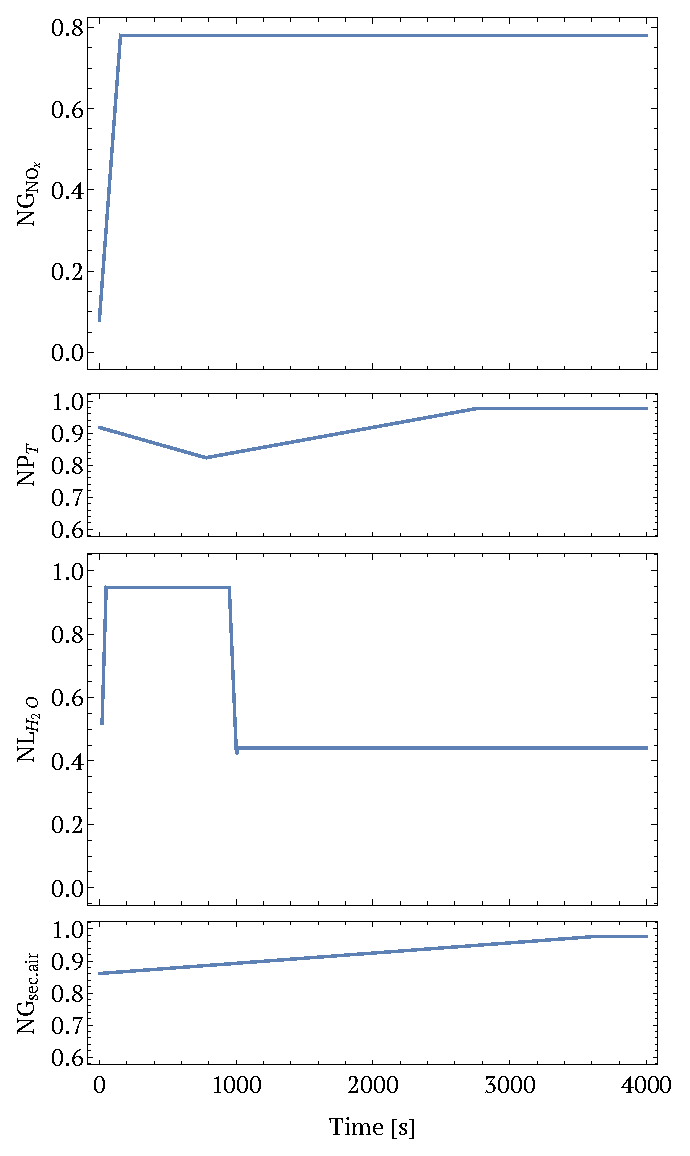
\includegraphics[width=0.7\textwidth]{figure2sp.eps}
	\caption[Sequence of ramps of the start-up procedure.]{Sequence of ramps of the start-up procedure: the first plot corresponds to the column's inlet \nox~gas flowrate, $NG_{\text{\nox}}$, the second to the inlet column's pressure, $NP_T$, the third to the column's inlet water flowrate, $NL_{\text{\hdoiso}}$, and the last one to the secondary air flowrate, $NG_{\text{sec.air}}$.} 
	\label{fig:modelall}
\end{figure}

\section{Dynamic process response -- additional information}
\label{s2:SI}

The effects of the lateral feed stream flow rate and secondary air flow rate during the column's startup are herein presented. Figure \ref{fig:startLinl} represents the simulation results for the reference scenario and for a scenario where the flow rate is reduced by \SI{30}{\percent}.
\begin{figure}[htb]
	\centering
	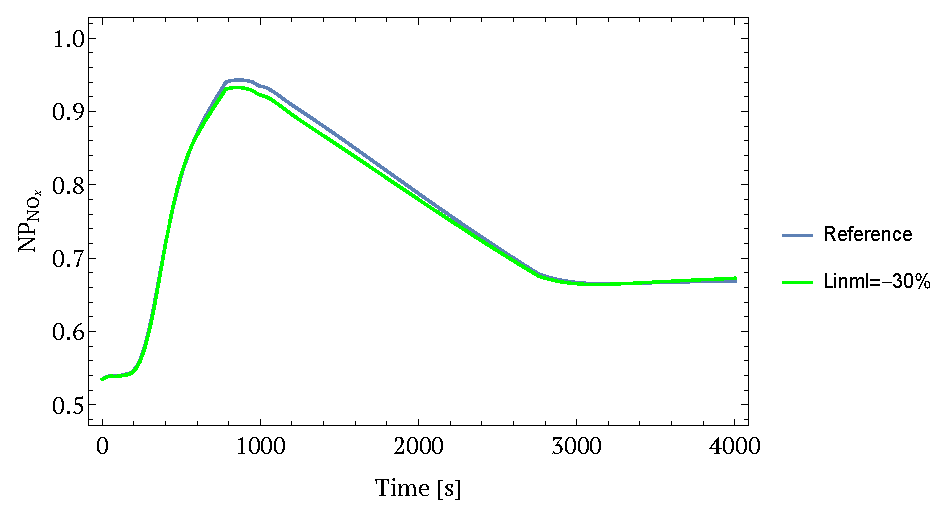
\includegraphics[width=0.8\textwidth]{figure3sp.eps}
	\caption{Comparison of the \nox~gas pressure leaving the column between the reference case and in case the lateral feed stream flow rate is reduced by  \SI{30}{\percent}.} 	
	\label{fig:startLinl}
\end{figure}
The analysis of Figure \ref{fig:startLinl} reveals that no considerable impact occurs when reducing the lateral feed stream flow rate by \SI{30}{\percent}; specifically, a decrease of \SI{1.3}{\percent} is observed at the peak. Figure \ref{fig:startLinlperfil} presents the nitric acid mass fraction profile at the beginning and end of startup. Observing the figure, we can conclude that decreasing the lateral feed stream flow rate will lead to an increase in the absorption rate in Zone 1, compared to the reference case, and consequently, the \hnotres~concentration is lower in the lateral feed tray. However this reduction is not significant and in Zone 2 the nitric acid profile is similar to that of the reference. Thus, low impact is observed in the \nox~gas stream leaving the column.


\begin{figure}[htb]
	\centering
	\includegraphics[width=0.8\textwidth]{figure4sp.eps}
	\caption{Nitric acid mass fraction profile in the beginning and end of startup in case the lateral stream flow rate is reduced by \SI{30}{\percent}.} 	
	\label{fig:startLinlperfil}
\end{figure}


The impact of the secondary air flow rate was also analysed, by simulating an increase of \SI{33.3}{\percent} with a normalized ramp slope of $1.6 \times 10^{-5}$ s$^{-1}$, from $t_2$ until $t_7$, as opposed to the reference scenario where an increase of \SI{13.4}{\percent} with a normalized ramp slope of $6.3 \times 10^{-6}$ s$^{-1}$ was used.
After the ramp, the secondary air flow rate was kept constant for the remaining period.
The comparison of the \nox~gas leaving the column between the reference case and this new scenario is shown in Figure \ref{fig:startair}.
\begin{figure}[htb]
	\centering
	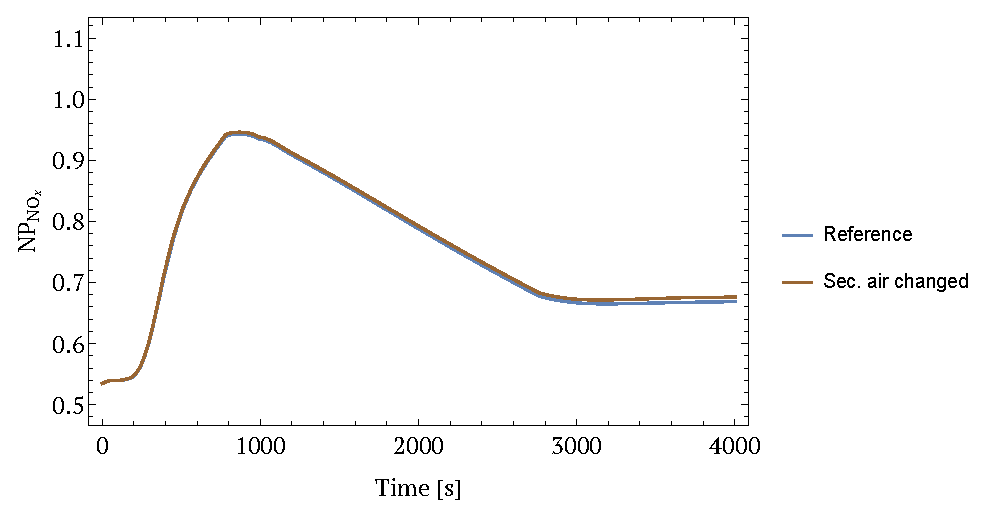
\includegraphics[width=0.8\textwidth]{figure5sp.eps}
	\caption{Comparison of the \nox~gas pressure leaving the column between the reference case and in case the secondary air has a different ramp profile.} 	
	\label{fig:startair}
\end{figure}
The dynamics do not show significant differences in the \nox~gas concentration leaving the column during the startup. 
The secondary air flow rate has an impact in the \no~oxidation rate as it increases the oxygen content in the inlet gas stream. This increase induces a higher oxidation rate which promotes the increase of the \nox~absorption rate, verified in Figure \ref{fig:startairperfil} where the beginning and end of startup profiles are analysed.

Figure \ref{fig:startairperfil} shows the influence of increasing the secondary air flow rate along the column and, in this case, no difference is observed when compared to the reference. Consequently, the increase of the secondary air does not have a significant impact on the \nox~pressures leaving the absorption column. Notice that, in this case, the mass fraction in Zone 1 is above 0.3 not causing any safety problems.




\begin{figure}[htb]
	\centering
	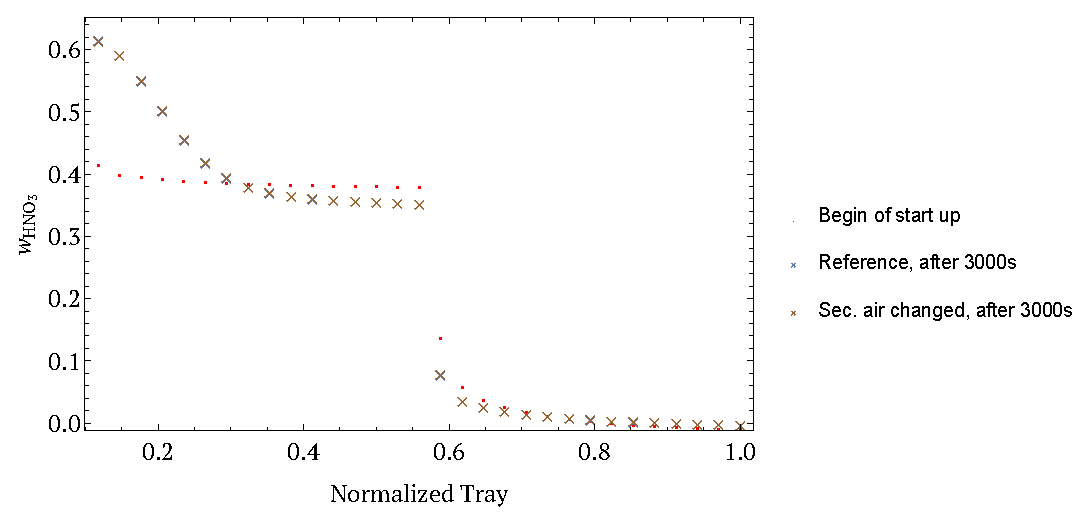
\includegraphics[width=0.8\textwidth]{figure6sp.eps}
	\caption{Nitric acid mass fraction profile in the absorption column at the beginning and end of startup in case the secondary air has a different ramp profile.} 	
	\label{fig:startairperfil}
\end{figure}






\bibliography{ACS-dynamicSI}







\end{document}
